\pdfoutput=1
\documentclass[11pt]{article}
\usepackage[margin=1in]{geometry}
\usepackage{newtxtext,newtxmath}
\usepackage{graphicx}
\usepackage{booktabs}
\usepackage{longtable}
\usepackage[round]{natbib}
\usepackage[hidelinks]{hyperref}
\usepackage{microtype}
\usepackage{caption}
\captionsetup{font=small,labelfont=bf}

\title{\Large\bfseries Evaluating the Relationship Between Diet \\ Affordability and Diet Quality: A Cross-Country Analysis of CoAHD and MDD-W}
\author{Nicholas E.\ Johnson \\ \small \texttt{nejohnson2@gmail.com}}
\date{September 2026}

\begin{document}
\maketitle

\begin{abstract}
\noindent
The 2026 \emph{State of Food Security and Nutrition in the World} (SOFI) reports both the share of each country's population unable to afford a healthy diet (the CoAHD indicator PUA) and, for the first time under the SDG framework, the share of women aged 15--49 achieving minimum dietary diversity (MDD-W, SDG indicator 2.2.4). We match the two indicators in the same calendar year for the 66 countries with both. Affordability explains roughly two thirds of the cross-country variation in women's dietary diversity, with each additional percentage point of unaffordability associated with a 0.71-point decline in MDD-W (95\% bootstrap CI $-0.82$ to $-0.60$; $R^2=0.65$). To address income confounding, we re-estimate the model with log GDP per capita included and find that unaffordability retains a coefficient of $-0.44$ ($p<10^{-4}$). Separately, the cost of a healthy diet in PPP dollars per day is uncorrelated with MDD-W ($R^2=0.00$) indicating that the relationship lies in cost relative to income rather than in the price level.  We use the remaining third of the variation, a residual standard deviation of 14 percentage points, as a descriptive benchmark for the \emph{non-price} constraints on diet quality. Three countries fall outside the 95\% prediction interval: Indonesia and Armenia above, Burkina Faso below. The analysis also shows that, where a country is measured by both platforms within two years, MDD-W estimates from the Gallup-based Global Diet Quality Project exceed DHS estimates by up to 20--30 percentage points, consistent with recent evidence that estimates from the two platforms are not directly comparable. These results provide evidence that making healthy diets affordable is a powerful predictor of women's dietary diversity, but a third of the gap between countries lies beyond the reach of price alone.
\end{abstract}

\medskip
\noindent\textbf{Keywords:} [AUTHOR INPUT REQUIRED: 4--6 keywords, e.g.\ diet cost; dietary diversity; MDD-W; food security]

\section{Introduction}\label{sec:intro}

Two indicators anchor the international monitoring of diets. The first is the Cost and Affordability of a Healthy Diet (CoAHD), an economic indicator that prices the least expensive locally available diet that meets food-based dietary guidelines and asks what share of each country's population cannot afford it \citep{herforth2020, bai2021}. The second is the Minimum Dietary Diversity for Women indicator (MDD-W), a dietary indicator that asks whether a woman of reproductive age consumed at least five of ten defined food groups in the previous day and night, a validated proxy for micronutrient adequacy \citep{arimond2010, martinprevel2015, fao2021}. The 2026 \emph{State of Food Security and Nutrition in the World} (SOFI) report elevates MDD-W to the SDG monitoring framework as indicator 2.2.4 \citep{fao2026}, so that for the first time both the economic constraint and a population-level diet-quality outcome are reported side by side for a substantial set of countries.

Given the availability of these two indicators, an assessment of their relationship can provide important information for food security efforts. If unaffordability entirely explains dietary diversity, lowering the cost of a healthy diet would be close to a sufficient policy.  Alternatively, if it explains very little, cost would be a distraction. Indeed, the 2026 SOFI report highlights that while reducing the cost of a healthy diet is necessary, it may not be sufficient to ensure diet diversity.  Using available data, this analysis aims to provide quantifiable evidence of the relationship between the two indicators and establish a benchmark with which to situate countries on either side.

This paper makes three contributions. First, we construct a same-year panel of the two indicators for 66 countries. Second, we estimate the affordability--diversity relationship and characterize its residual as a benchmark for which countries achieve substantially more dietary diversity than their affordability predicts, and which achieve less. Third, we identify important measurement weaknesses. The SDG 2.2.4 series mixes three survey platforms---the Gallup World Poll modules of the Global Diet Quality Project (GDQP), the Demographic and Health Surveys (DHS), and one-off national surveys---whose estimates are not directly comparable \citep{hanleycook2025}. We compile survey-level metadata (sampling frame, mode, fieldwork window, documented geographic exclusions) for every observation in the panel in order to flag the surveys with material coverage limitations and conduct sensitivity analyses that account for these differences.

Section~\ref{sec:related} situates the analysis in the literature; Section~\ref{sec:data} describes the data and sample; Section~\ref{sec:methods} sets out the model and sensitivity tests; Section~\ref{sec:results} reports results; Section~\ref{sec:discussion} discusses interpretation and limitations.

\section{Related work}\label{sec:related}

Three strands of literature frame the analysis. The first develops the cost and affordability of healthy diets as a measurable object: least-cost diet methods and price indexes for diet quality \citep{masters2018}, the global CoAHD estimates that underlie SOFI \citep{herforth2020, bai2021}, and evidence that the price of nutritious foods relative to staples rises systematically as incomes fall \citep{headey2019}. This strand established that healthy diets are unaffordable for billions and argued, largely from price and income data, that affordability binds diet quality. Direct cross-country tests of that proposition against a measured population-level diet-quality outcome remain scarce [CITATION NEEDED: any prior study regressing a national diet-quality indicator on CoAHD-style affordability], which is the gap this paper addresses.

The second strand develops and validates the outcome measure. MDD-W originates in multi-country validation studies showing that simple food-group counts predict the micronutrient adequacy of women's diets \citep{arimond2010}, was standardized as an operational indicator \citep{martinprevel2015}, codified in FAO's measurement guide \citep{fao2021}, and elevated to SDG indicator 2.2.4 in the 2026 monitoring cycle \citep{fao2026}.

The third strand concerns measurement comparability. \citet{hanleycook2025} compare contemporaneous DHS and Gallup World Poll MDD-W estimates and find differences exceeding five percentage points in every country-year set examined, traceable to divergent sentinel-food lists, fieldwork windows, and languages; Gallup's own documentation records the sampling frames and geographic exclusions of each round \citep{gallup2024, gdqp}. This paper contributes to that strand a panel-wide compilation of survey metadata and an assessment of how far the platform mixture conditions cross-country inference.

\section{Data}\label{sec:data}

\subsection{Affordability}
The CoAHD indicators are taken from the FAOSTAT \texttt{CAHD} domain, July 2026 release (the SOFI 2026 vintage), which provides two related indicators \citep{faostat2026}. The first is the cost of a healthy diet (CoHD; item 70040). For each country, the cheapest combination of locally available foods that satisfies the national food-based dietary guidelines is identified at ordinary retail prices and expressed in PPP dollars per person per day.  While this is not actually a diet that anyone eats, it is designed to be the minimum a person in that country would have to spend to eat a healthy diet at all. CoHD is available from 2017 to 2025 for 166 countries.

The second CoAHD indicator is the prevalence of unaffordability (PUA; FAOSTAT item 7005), which is the share of the national population unable to afford a healthy diet.  PUA is computed using a country's income distribution after reducing household incomes by a standard non-food allowance, leaving the proportion of income realistically available for food consumption.  The income reduction is based on the assumption that households do not devote their entire income to food.  PUA is then the share of the population whose food-available income falls below the cost of the least-cost healthy diet.  PUA is available annually from 2017 to 2025 for 149 countries; its narrower coverage than CoHD reflects the additional requirement of a usable household income or consumption survey \citep{herforth2020}.

\subsection{Dietary diversity}
MDD-W is taken from the FAOSTAT \texttt{SDGB} domain, indicator 2.2.4, national series (item \texttt{24049-F-Y15T49T}) and defined as the percentage of non-pregnant women aged 15--49 achieving minimum dietary diversity. Seventy-nine countries have at least one observation (106 country-years, 2016--2025) and FAOSTAT records the underlying data collection source for every observation.  For this analysis, 67 country-years were derived from the GDQP \citep{gdqp}, 22 from DHS, and 17 from one-off national nutrition or food-security surveys. The years attached to these estimates are fieldwork years, not publication years, which is what permits same-year matching to CoAHD.

\subsection{Survey metadata and coverage flags}
For each MDD-W observation used in the panel we compiled fieldwork dates, sample size, design effect, interview mode, and documented geographic exclusions from Gallup's country data-set documentation \citep{gallup2024} and, for DHS and national surveys, from the FAOSTAT source notes. Three binary flags summarize material limitations: \emph{exclusion} ($\geq$10\% of the national population outside the sampling frame; five countries, up to 23\% excluded in Chad and 20\% in Cameroon); \emph{telephone frame} (landline/mobile samples, which under-cover households without phones; ten countries); and \emph{unverified} (one-off national surveys whose coverage we could not verify; six countries). Twenty-one of the 66 panel surveys carry at least one flag. The flags do not alter any estimate; they mark countries in the figures and define one sensitivity subsample.

\subsection{Covariates}
World Bank region and income-group classifications and GDP per capita at purchasing power parity (constant 2021 international dollars) complete the panel \citep{worldbank}.

\subsection{Panel construction}
For each country we take the most recent MDD-W survey and match the CoAHD estimate for the same calendar year; a $\pm$2-year fallback was specified in advance but never invoked---all 66 countries matched exactly. Countries are joined on ISO3 codes derived from FAOSTAT's M49 codes. Thirteen MDD-W countries lack any usable CoAHD estimate (Afghanistan, Cambodia, Georgia, Libya, Oman, Somalia, Tajikistan, Thailand, Timor-Leste, Ukraine, Vanuatu, Venezuela, Zimbabwe) and are dropped; every drop is logged. The resulting sample of 66 comprises 32 countries in Sub-Saharan Africa, 11 in Europe and Central Asia, 9 in the Middle East and North Africa, 6 each in East Asia--Pacific and Latin America, and 2 in South Asia; by income group, 15 low-income, 27 lower-middle, 21 upper-middle, and 3 high-income. Survey years run from 2018 (one country) through 2021--2024 (65 countries). Unaffordability spans 1.1\% (Switzerland) to 92.1\% (Malawi); MDD-W spans 17.2\% to 91.2\%. A second panel applies a source-priority rule---prefer a DHS or national survey over Gallup when one exists from 2018 onward---and differs in three countries (C\^ote d'Ivoire, Kyrgyzstan, Sierra Leone).

\subsection{Sample selection and missingness}\label{sec:missing}
Because the panel is the intersection of two incomplete series, it is worth asking who is missing and whether selection is adverse. Two comparisons address this. First, the 13 countries with an MDD-W estimate but no usable PUA do not differ detectably from the 66 retained: their most recent MDD-W values average 65.8 against the panel's 59.4 (Mann--Whitney $p=0.56$), and their income-group composition is similar. Second, and more consequentially, 149 countries publish a PUA estimate (147 once restricted to areas with standard ISO3 codes); the 81 of these excluded for lack of any MDD-W survey are concentrated at the \emph{affordable} end. Inclusion rates are 79\% for low-income countries, 73\% for lower-middle, 49\% for upper-middle, and 6\% for high-income, and the panel's mean unaffordability (45.0\%) is roughly double that of the excluded set (23.0\%; Mann--Whitney $p<10^{-4}$). Twenty of the 25 highest-unaffordability countries in the world are in the panel; the five exceptions are states without a recent diet survey, most of them crisis-affected (South Sudan, Haiti, the Central African Republic, Eswatini, Guinea-Bissau). The sample is therefore close to a census of the high-unaffordability world and sparse where unaffordability is lowest---selection on the explanatory variable, which limits extrapolation to the rich, low-PUA end but does not by itself bias the fitted slope within the observed range.

\section{Methods}\label{sec:methods}

The headline model is deliberately simple:
\begin{equation}
\mathrm{MDDW}_i \;=\; \alpha + \beta\,\mathrm{PUA}_i + \varepsilon_i,
\label{eq:main}
\end{equation}
estimated by ordinary least squares with heteroskedasticity-robust (HC3) standard errors and a 5{,}000-draw country-level bootstrap for the slope and $R^2$. The residual $\hat\varepsilon_i$ is the object of interest: dietary diversity higher or lower than affordability alone predicts. We read it as a descriptive benchmark---it bundles food availability, home production, preferences, urbanization, the season of the survey, conflict, and measurement error in both indicators---and deliberately avoid the language of ``performance'' or causal effects.

Three guards discipline the residual reading. Each country's benchmark is recomputed leaving that country out, yielding leave-one-out (LOO) residuals and a cross-validated $R^2$. ``Unusual'' is defined as lying outside the classical 95\% prediction interval, a far stricter criterion than merely missing the line. Countries are labelled in figures only when the externally studentized residual exceeds one in absolute value.

Sensitivity tests are organized by the objection each is designed to answer. Six appear in the main text (Table~\ref{tab:robust}):
\begin{itemize}
\item \emph{Income confounding} (PUA $+$ log GDP per capita). PUA and log GDP are correlated at $-0.78$; if the affordability coefficient collapsed once income entered, the relationship would be income in disguise.
\item \emph{Regional structure} (PUA $+$ region fixed effects). Countries in the same region share food environments, dietary patterns, and---not incidentally---survey platforms. Re-estimating within regions asks how much of the global relationship is between-region structure, and re-benchmarks each country against its neighbours rather than the world.
\item \emph{Platform offset} (PUA $+$ survey-source dummies). The SDG 2.2.4 series mixes Gallup, DHS, and national surveys whose estimates are not directly comparable \citep{hanleycook2025}; source dummies estimate that offset and test whether the slope survives it. Because platform assignment is not random---DHS-measured countries are systematically poorer---the dummy absorbs both instrument effects and any real differences between the country groups, and we read it as descriptive of the mixture rather than as a pure instrument effect.
\item \emph{Platform mixing} (GDQP-sourced countries only). If pooling incompatible platforms manufactured the correlation, it would vanish in a single-platform subsample, where estimates are internally comparable.
\item \emph{Survey coverage} (excluding all flagged surveys). The result should stand on the cleanest surveys alone: household sampling frames, no material exclusions, verified national coverage.
\item \emph{Out-of-sample validity} (leave-one-country-out cross-validation). With 66 observations, in-sample fit can flatter; predicting each country from a model that never saw it yields an honest $R^2$, and residuals in which no country helps set its own benchmark.
\end{itemize}
Seven further tests, reported in Appendix~\ref{app:sens} with the purpose of each, probe analytic choices that turn out to be immaterial: the bounded outcome, functional form, the complementary platform subsample, sampling precision, the year-matching rule, influential observations, and the survey-selection rule. Where a test defines residuals, we report the Spearman rank correlation between its residuals and the headline residuals.

All data are public; the pipeline (download, panel construction, estimation, figures) is four short Python scripts with a fixed seed, and figures read only from saved results.

\section{Results}\label{sec:results}

\subsection{Affordability explains about two thirds}\label{sec:headline}

Figure~\ref{fig:main} shows the relationship, and it is a strong one. The fitted line is $\mathrm{MDDW} = 92.7 - 0.71\,\mathrm{PUA}$: a country in which no one is priced out of a healthy diet is predicted to have about 93\% of women meeting the MDD-W threshold, and a country in which everyone is priced out, about 22\%. The slope's 95\% bootstrap confidence interval is $(-0.82, -0.60)$; $R^2$ is $0.65$ (bootstrap CI $0.50$--$0.78$), and the leave-one-country-out $R^2$ of $0.63$ shows the fit is not carried by any single observation. Forty-four of 66 countries lie within one residual standard deviation (14.1 points) of the line, and the residuals pass standard diagnostics (Breusch--Pagan $p=0.35$; Shapiro--Wilk on studentized residuals $p=0.57$).

A word about the shaded band in Figure~\ref{fig:main} is warranted, because it is deliberately \emph{not} a confidence or prediction interval. The band marks $\pm$1 residual standard deviation and answers a descriptive question: how large is a typical miss? By construction, roughly a third of countries should fall outside such a band when residuals are approximately normal, and 22 of 66 do---close to the 21 expected---so countries outside it are not anomalies but simply larger-than-typical deviations, and the band serves as a ruler for grading them. The formal criterion for an \emph{unusual} country is the 95\% prediction interval defined in Section~\ref{sec:methods}, which is roughly twice as wide because it asks a different question: where could a new country plausibly fall, given the fitted relationship and the scatter around it? Only three countries escape that interval---Indonesia and Armenia above, Burkina Faso below. We display the tighter band rather than the prediction interval because a band that contains 63 of 66 points would render the figure uninformative; the $\pm$1~SD ruler lets the reader distinguish moderate deviations from the handful of large ones. A restricted cubic spline does not improve on the straight line ($F$-test $p=0.18$), and the fractional logit ranks countries identically to OLS (Spearman $\rho=0.99$), so we report the linear model for interpretability. Two objections arise immediately---that the gradient merely restates national income, and that it is an artifact of how MDD-W is measured. Sections~\ref{sec:income} and~\ref{sec:platform} take these in turn.

\begin{figure}[tbp]
\centering
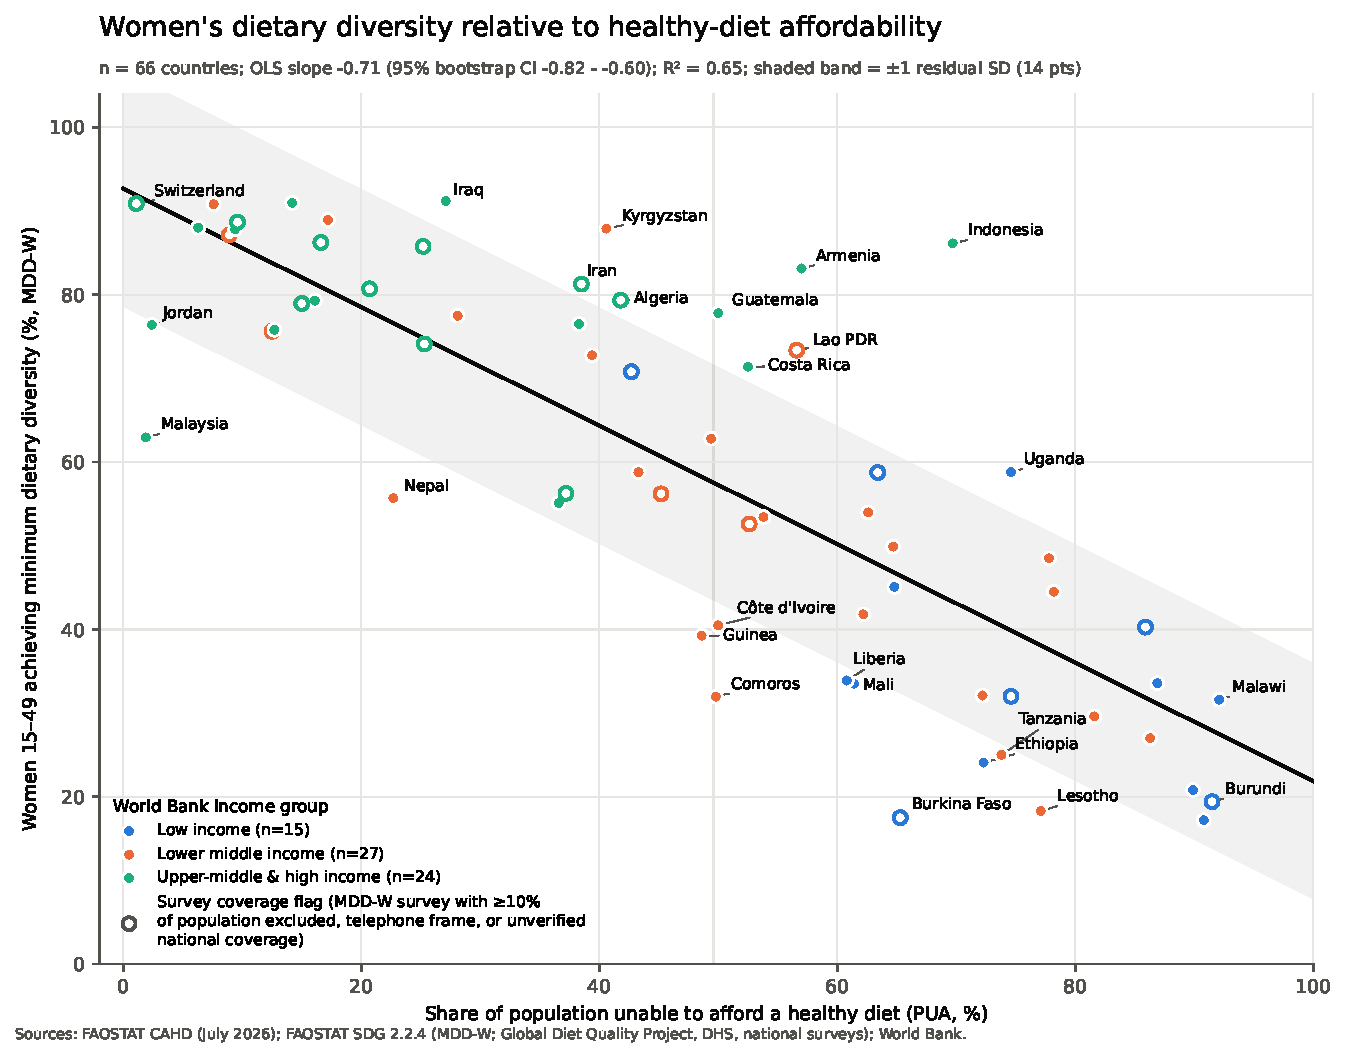
\includegraphics[width=\textwidth]{fig1_affordability_quality_gap.pdf}
\caption{Women's dietary diversity against the share of the population unable to afford a healthy diet, 66 countries, indicators matched in the survey year. The line is the OLS fit; the band is $\pm$1 residual standard deviation---a descriptive ruler for the size of deviations, not a confidence interval, so roughly a third of countries are expected to lie outside it (see Section~\ref{sec:headline}). Colour denotes World Bank income group; hollow markers denote surveys with a documented coverage limitation ($\geq$10\% of the population excluded from the frame, a telephone frame, or unverified national coverage). Countries with $|$studentized residual$|>1$ are labelled.}
\label{fig:main}
\end{figure}

\subsection{Not income, and not the price level}\label{sec:income}

Log GDP per capita alone explains 62\% of the variance in MDD-W and is correlated with PUA at $-0.78$, so one must ask whether the affordability relationship is simply income. It is not. With both regressors included, PUA retains a coefficient of $-0.44$ (HC3 $p<10^{-4}$) while log GDP contributes 9.6 points per log unit ($p=0.002$), and $R^2$ rises only from 0.65 to 0.71. At a given income level, countries where healthy diets are more affordable have measurably more diverse diets---precisely what an indicator designed to capture the price--income relationship, rather than income per se, should deliver. The headline residual is only weakly correlated with income ($r=0.26$), so the non-price component is not relabelled GDP either.

A sharper decomposition is possible because CoAHD reports both the cost level and its affordability. The cost of a healthy diet in PPP dollars per day is essentially uncorrelated with MDD-W across countries ($R^2=0.00$) and contributes nothing alongside PUA. The signal resides entirely in cost \emph{relative to income}. This is consistent with the observation that nutritious foods are cheap in poor agricultural economies in absolute terms yet unaffordable relative to incomes \citep{headey2019, masters2018}.

\subsection{Regional structure}\label{sec:region}

Geography does real work in this relationship. Region fixed effects raise $R^2$ to 0.78 and attenuate the PUA slope to $-0.39$ (still $p=0.001$). At the same level of unaffordability, Sub-Saharan Africa's intercept sits roughly 22 points below the East Asia--Pacific reference and South Asia's about 18 points below, while Europe--Central Asia, Latin America, and MENA are statistically indistinguishable from it. Part of what the bivariate model attributes to affordability is therefore broad regional structure---food environments, dietary patterns, and, not incidentally, survey platforms differ by region in ways PUA does not capture. The practical consequence is that some countries look unusual against the global line but ordinary against their region: Guatemala ($+21$ globally, $+5$ within region), Costa Rica ($+16$, $-1$), Peru ($+11$, $-1$), and Nepal ($-21$, $-6$). Others hold their position under both benchmarks: Indonesia ($+43$, $+25$), Armenia ($+31$, $+14$), Kyrgyzstan ($+24$, $+12$), Uganda ($+19$, $+22$), and Iraq ($+18$, $+14$) above; Malaysia ($-28$, $-24$), Burkina Faso ($-29$, $-23$), Lesotho ($-20$, $-18$), and Mongolia ($-12$, $-19$) below. We treat a country as a candidate for case study only when it is far from the line under both benchmarks and its survey carries no coverage flag.

\subsection{The residual benchmark}\label{sec:resid}

Figure~\ref{fig:league} turns the residuals into a league table: all 66 countries, ordered by how far they sit from the affordability benchmark. Splitting at the median unaffordability (49.6\%) and at the fitted line yields four descriptive groups, which we phrase as higher or lower MDD-W than predicted---not as performance.

\emph{Higher unaffordability, MDD-W above prediction} ($n=14$). Fourteen countries deliver more dietary diversity than their high unaffordability predicts. Indonesia is the most striking: 70\% of the population is assessed as unable to afford a healthy diet, yet 86\% of women meet the MDD-W threshold, 43 points above prediction and outside the 95\% prediction interval, on an unflagged face-to-face survey. Armenia ($+31$, also outside the interval), Lao PDR ($+21$; Gallup excluded 14\% of the population---flagged), Guatemala ($+20$), and Uganda ($+19$) follow.

\emph{Lower unaffordability, MDD-W below prediction} ($n=15$). This quadrant is the empirical content of SOFI's caveat: healthy diets are comparatively affordable, yet diversity falls short. Malaysia is the sharpest case---1.9\% priced out, 63\% MDD-W, 28 points below prediction under both the global and regional benchmarks, on an unflagged survey. Nepal ($-21$ globally, though only $-6$ within South Asia; DHS) and Jordan ($-15$; DHS) are the other labelled members. Here the binding constraint is evidently not price.

\emph{Higher unaffordability, MDD-W below prediction} ($n=19$). Dominated by Sub-Saharan Africa, this is the quadrant where both constraints bind at once. Burkina Faso shows the largest negative deviation ($-29$, outside the prediction interval), but its estimate derives from a 2023 SMART nutrition survey whose national coverage we could not verify; it is flagged and should not be quoted without that qualification. Comoros ($-26$), Lesotho ($-20$; DHS), Guinea ($-19$), Ethiopia ($-17$; the Gallup round excluded Tigray, Gambella, and Harari), C\^ote d'Ivoire, Liberia, Mali, and Tanzania ($-15$ to $-17$) complete the group. The fourth quadrant---lower unaffordability with diversity at or above prediction ($n=18$)---is the unremarkable case where price and diet align, and needs no commentary.

\begin{figure}[tbp]
\centering
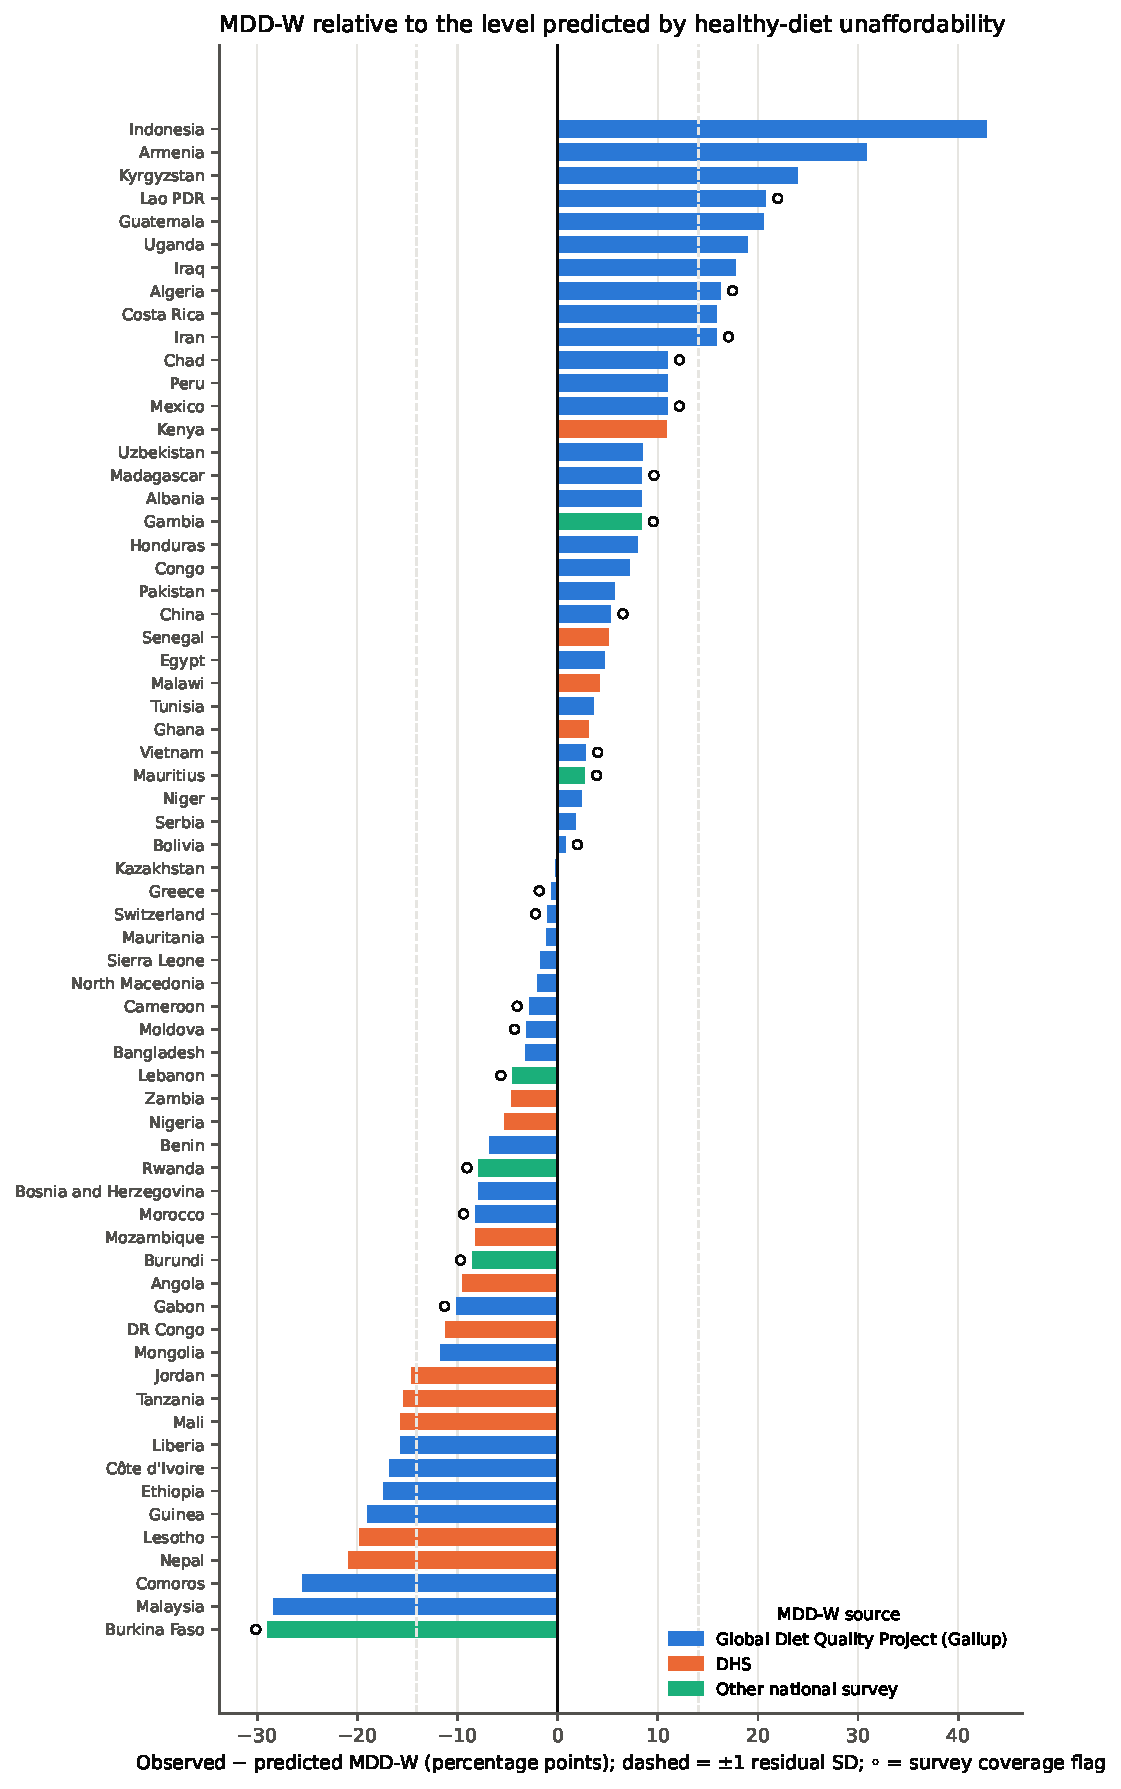
\includegraphics[width=.8\textwidth]{fig2_residual_league_table.pdf}
\caption{Observed minus predicted MDD-W (percentage points), all 66 countries, ordered by residual. Bar colour denotes the survey platform behind the MDD-W estimate; open circles mark surveys with a documented coverage limitation. Dashed lines are $\pm$1 residual standard deviation.}
\label{fig:league}
\end{figure}

\subsection{The survey-platform problem}\label{sec:platform}

Figure~\ref{fig:bysource} repeats Figure~\ref{fig:main} with points coloured by survey platform, and the pattern is immediate: DHS-sourced points cluster on or below the line, and nearly every large positive residual is Gallup-sourced. Where a country appears in the SDG series with estimates from both platforms no more than two years apart, the GDQP figure is higher in 10 of 11 such pairs: by 32 points in the Democratic Republic of the Congo, 31 in Mozambique, 25 in Mali, 21 in Malawi and Kenya, and 12 in Senegal (Table~\ref{tab:dual}; the three pairs separated by four or more years confound platform differences with real change and are shown for completeness only). Differences of this size over one or two years are not plausible dietary change. They are consistent with the head-to-head comparison of \citet{hanleycook2025}, who find that contemporaneous DHS and Gallup World Poll estimates differ by more than five points in every one of nine country-year sets examined (range $-17$ to $+21$), that the sentinel-food lists underlying the two questionnaires overlap by only 21--65\% within the same country, and that Gallup fieldwork spans fewer months in fewer languages; they conclude the platforms cannot currently be calibrated to one another. Because MDD-W is a threshold indicator---one additional ``yes'' among ten food groups moves a respondent across the 5-group cutoff---modest differences in food lists and probing translate into large differences in the share above threshold. Seasonal timing compounds the problem: a Gallup round typically spans three to six weeks where a DHS spans several months, and single-year dietary diversity is known to swing substantially across the agricultural calendar \citep{hanleycook2025, fao2021}.

What does this mean for the analysis? Three things. First, the slope is attenuated but not overturned by platform adjustments: $-0.62$ with source dummies, $-0.59$ in the GDQP-only subsample (whose lower $R^2$ of 0.51 partly reflects the narrower unaffordability range that subsample spans), $-0.69$ in the DHS/national-only subsample, $-0.68$ excluding all 21 flagged surveys, and $-0.70$ on the source-priority panel (Tables~\ref{tab:robust} and~\ref{tab:sensx}). In the pooled model, DHS-sourced observations sit 12.8 points below GDQP-sourced observations at the same level of unaffordability ($p=0.002$). Second, the residual \emph{ranking} is robust: Spearman correlations with the headline residuals are 0.92 (source dummies), 0.98 (latest-year PUA), 0.999 (precision weights), and 0.998 (excluding flagged surveys). Third, individual countries do move. Once source is adjusted, Jordan's residual improves from $-15$ to $-1$, Senegal's from $+5$ to $+14$, and Kenya's from $+11$ to $+17$. The large positive outliers named in Section~\ref{sec:resid} are almost all GDQP-sourced and hence internally comparable; the negative outliers are mixed-source, and comparisons among them should be treated as approximate.

\begin{figure}[tbp]
\centering
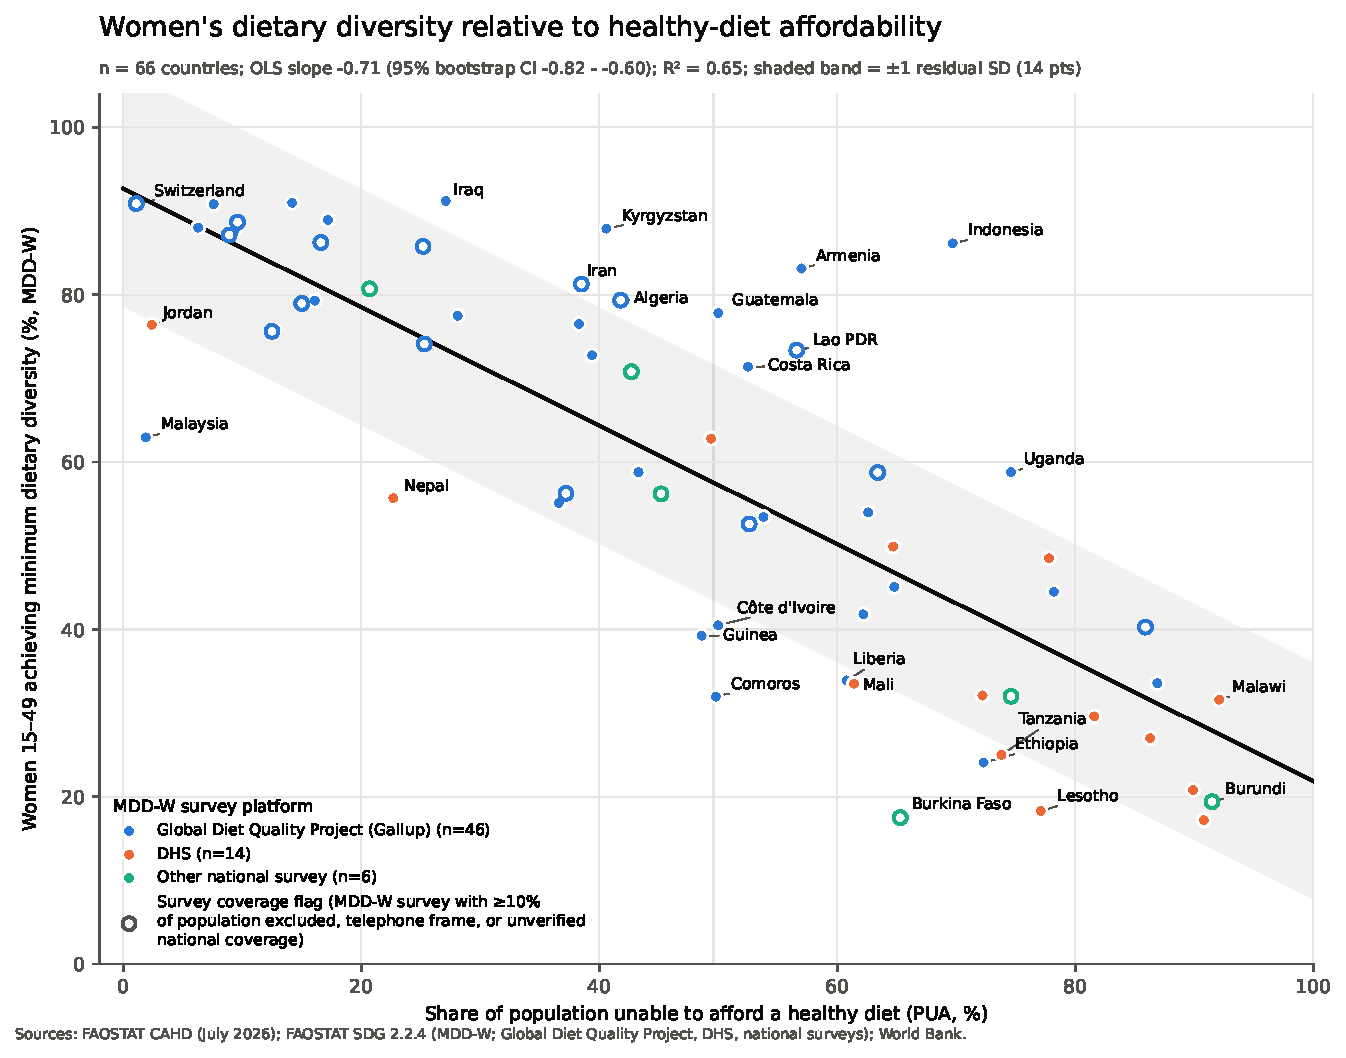
\includegraphics[width=\textwidth]{fig1b_affordability_quality_gap_by_source.pdf}
\caption{As Figure~\ref{fig:main}, with colour denoting the survey platform behind each MDD-W estimate. DHS-sourced estimates (orange) sit systematically at or below the fitted line; nearly all large positive deviations are Gallup-sourced (blue).}
\label{fig:bysource}
\end{figure}

\begin{table}[tbp]
\centering\small
\caption{Countries with MDD-W estimates from more than one platform in the SDG 2.2.4 series (panel countries only). Among the 11 pairs measured no more than two years apart, the GDQP estimate is higher in 10; the three pairs separated by four or more years (Uzbekistan, Sierra Leone, Mongolia) confound platform differences with real dietary change and are included for completeness only.}
\label{tab:dual}
\begin{tabular}{lcccr}
\toprule
Country & GDQP estimate & Household-survey estimate & Years & Gap (pp)\\
\midrule
Uzbekistan & 88.9 & 40.4 (national) & 2022 / 2017 & $+48.5$\\
DR Congo & 49.0 & 17.2 (DHS) & 2023 / 2024 & $+31.8$\\
Mozambique & 51.6 & 20.8 (DHS) & 2021 / 2023 & $+30.8$\\
Mali & 58.0 & 33.5 (DHS) & 2022 / 2024 & $+24.5$\\
Malawi & 53.1 & 31.6 (DHS) & 2023 / 2024 & $+21.4$\\
Kenya & 69.3 & 48.5 (DHS) & 2021 / 2022 & $+20.8$\\
Kyrgyzstan & 87.9 & 69.5 (national) & 2022 / 2021 & $+18.4$\\
Senegal & 74.8 & 62.8 (DHS) & 2021 / 2023 & $+12.0$\\
C\^ote d'Ivoire & 40.5 & 29.4 (DHS) & 2023 / 2021 & $+11.1$\\
Nepal & 63.9 & 55.7 (DHS) & 2021 / 2022 & $+11.0$\\
Tanzania & 35.9 & 25.0 (DHS) & 2021 / 2022 & $+10.9$\\
Ghana & 44.1 & 49.9 (DHS) & 2021 / 2022 & $-5.8$\\
Sierra Leone & 45.1 & 56.4 (DHS) & 2023 / 2019 & $-11.3$\\
Mongolia & 55.1 & 70.2 (national) & 2023 / 2016 & $-15.1$\\
\bottomrule
\end{tabular}
\end{table}

\subsection{Sensitivity summary}

Table~\ref{tab:robust} reports the six main sensitivity tests; Appendix~\ref{app:sens} reports seven more. Across all thirteen, the affordability slope lies between $-0.59$ and $-0.76$ and is always significant at conventional levels, and the residual ranking correlates with the headline at $\rho\geq0.96$ in every test except region fixed effects ($\rho=0.79$)---the one specification that deliberately changes the question, from a global benchmark to a within-region one. The tests capable of overturning the result (income, platform, coverage) attenuate the slope only modestly; the tests of analytic choices (functional form, year matching, weighting, influence) move it by at most $0.05$.

\begin{table}[tbp]
\centering\small
\caption{Main sensitivity tests. Each row answers the objection stated in Section~\ref{sec:methods}. The final column is the Spearman correlation between the test's residuals and the headline residuals, where defined. Seven additional sensitivity tests appear in Appendix~\ref{app:sens}.}
\label{tab:robust}
\begin{tabular}{llrrrrr}
\toprule
Objection addressed & Sensitivity test & $n$ & PUA coef. & (SE) & $R^2$ & $\rho$(resid)\\
\midrule
--- & OLS, headline & 66 & $-0.71$ & (0.06) & 0.65 & ---\\
Income confounding & PUA $+$ log GDP & 66 & $-0.44$ & (0.11) & 0.71 & ---\\
Regional structure & PUA $+$ region fixed effects & 66 & $-0.39$ & (0.12) & 0.78 & 0.79\\
Platform offset & PUA $+$ source dummies & 66 & $-0.62$ & (0.06) & 0.70 & 0.92\\
Platform mixing & GDQP-sourced only & 46 & $-0.59$ & (0.08) & 0.51 & ---\\
Survey coverage & Exclude flagged surveys & 45 & $-0.68$ & (0.08) & 0.60 & 0.998\\
Out-of-sample validity & Leave-one-country-out CV & 66 & --- & --- & 0.63 & 1.00\\
\bottomrule
\end{tabular}
\end{table}

\section{Discussion}\label{sec:discussion}

\subsection{What the residual is, and is not}
The residual from equation~(\ref{eq:main}) is a descriptive quantity: the part of women's dietary diversity that a single affordability number does not predict. It aggregates the density and reach of food retail, home production and informal markets, cultural dietary patterns, women's time and intra-household allocation, nutrition knowledge and programming, the season of the survey, and conflict, together with measurement error in both indicators. With 66 observations we make no attempt to decompose it. Its value is as a targeting device. Where a country sits far below the benchmark at low unaffordability---Malaysia is the cleanest case---``make healthy diets cheaper'' is aimed at the wrong margin, and attention belongs on the demand side and the food environment. Where a country sits far above the benchmark at high unaffordability---Indonesia, Uganda---something in the food system delivers diversity at price points the affordability metric scores as out of reach, and understanding that mechanism is worth field study. One candidate mechanism deserves emphasis: PUA prices the least-cost diet at \emph{retail} and compares it with \emph{measured income}, so in agricultural economies with substantial own-production, subsistence consumption bypasses both sides of that comparison, and market-based unaffordability will overstate the effective constraint on diet quality. The fact that the residual is essentially uncorrelated with the price \emph{level} of a healthy diet, and only weakly with income, sits comfortably with this reading.

\subsection{Implications for monitoring}
The platform findings carry a monitoring lesson independent of the affordability question. The new SDG 2.2.4 series is, at present, a mixture of instruments that differ by amounts (10--30 points within country) far exceeding any plausible real change over the intervals involved. Until harmonization or calibration advances, three practices seem prudent: publish the platform alongside every national estimate; never infer trends across a platform switch; and accompany cross-country league tables with source flags of the kind used here. None of this diminishes the value of the indicator---our DHS-only subsample reproduces the affordability relationship almost exactly---but it does mean that individual country rankings inherit the measurement system's present limitations.

\subsection{Limitations}
The usual cautions apply here with more than usual force. The analysis is cross-sectional, with one observation per country, and supports no causal claim in either direction; diets and incomes are jointly determined. MDD-W describes women aged 15--49 and proxies micronutrient adequacy, not diet quality generally, while PUA describes the entire population---the two indicators do not cover the same people. CoAHD is a modelled indicator whose assumptions (a fixed least-cost guideline diet, a non-food expenditure allowance, retail prices) carry through. The panel is thin at the top of the income distribution (three high-income countries), so ``lower unaffordability'' here means below a median of roughly 50\%, not affordable in an absolute sense. The precision weights rest on documented but approximate effective sample sizes rather than published standard errors. Finally, the survey-platform heterogeneity discussed throughout bounds the confidence one should place in any single country's residual, even where our flags are clean.

Sample selection, examined in Section~\ref{sec:missing}, appears benign on observables: the countries lost to missing data do not differ detectably in dietary diversity or income from those retained, and the panel captures nearly all of the world's highest-unaffordability countries. The important qualification runs the other way---high-income, low-unaffordability countries are largely absent because they field no MDD-W surveys---so the benchmark should not be extrapolated to that end of the distribution.

\section{Conclusion}\label{sec:conclusion}

Across 66 countries, the share of the population unable to afford a healthy diet explains about two thirds of the variation in the share of women achieving minimum dietary diversity---a relationship that survives controls for income, region, survey platform, sampling precision, and coverage limitations, and that reflects affordability specifically rather than the price level. The remaining third is a 14-point residual standard deviation with interpretable structure: a small set of countries sits far above or below the affordability benchmark under every specification tried. That is the empirical content of SOFI's own caveat that reducing the cost of healthy diets, while necessary, will not by itself close the diet-quality gap, and it identifies where the non-price constraints---and the non-price successes---are most worth studying. It is equally a demonstration that the new global MDD-W series is not yet platform-harmonized, and that country-level inferences from it should carry the survey's provenance alongside the number.

\subsection*{Disclosure of AI assistance}
In accordance with arXiv's policy on the use of generative AI tools, the author discloses that an AI assistant (Claude, Anthropic) was used substantially in this work: to write the data-processing and analysis code, to generate the figures, and to draft the manuscript text. The author specified the research question, design, and analytic choices; reviewed the code, data handling, and all reported numbers; and verified the references. Responsibility for the content rests entirely with the author.

\subsection*{Reproducibility}
All inputs are public (FAOSTAT bulk downloads, World Bank API, Gallup survey documentation). The full pipeline---download, panel construction with logged exclusions, estimation, and figures---is available at [AUTHOR INPUT REQUIRED: repository URL or archive DOI]; a fixed seed reproduces every number in this paper, and the compiled survey-coverage metadata are distributed with the code.

\bibliographystyle{plainnat}
\begin{thebibliography}{99}

\bibitem[Arimond et~al.(2010)]{arimond2010}
Arimond, M., Wiesmann, D., Becquey, E., Carriquiry, A., Daniels, M.~C., Deitchler, M., Fanou-Fogny, N., Joseph, M.~L., Kennedy, G., Martin-Pr\'evel, Y., and Torheim, L.~E. (2010).
Simple food group diversity indicators predict micronutrient adequacy of women's diets in 5 diverse, resource-poor settings.
\emph{Journal of Nutrition}, 140(11):2059S--2069S.

\bibitem[Bai et~al.(2021)]{bai2021}
Bai, Y., Alemu, R., Block, S.~A., Headey, D., and Masters, W.~A. (2021).
Cost and affordability of nutritious diets at retail prices: Evidence from 177 countries.
\emph{Food Policy}, 99:101983.

\bibitem[FAO(2021)]{fao2021}
FAO (2021).
\emph{Minimum dietary diversity for women: An updated guide to measurement---from collection to action}.
FAO, Rome.

\bibitem[FAO et~al.(2026)]{fao2026}
FAO, IFAD, UNICEF, WFP, and WHO (2026).
\emph{The State of Food Security and Nutrition in the World 2026}.
FAO, Rome.

\bibitem[FAOSTAT(2026)]{faostat2026}
FAOSTAT (2026).
Domains CAHD (Cost and Affordability of a Healthy Diet, July 2026 release) and SDGB (SDG indicators).
Bulk downloads: \url{https://bulks-faostat.fao.org/production/datasets_E.json}.

\bibitem[Gallup(2024)]{gallup2024}
Gallup (2024).
\emph{Country data set details: DQQ, Gallup worldwide research data collected 2021--2024}.
\url{https://www.dietquality.org/DQQ\%20data\%20collection\%20details\%20GWP\%202021-2024.pdf}.

\bibitem[Global Diet Quality Project(2024)]{gdqp}
Global Diet Quality Project (2024).
Diet quality data.
Harvard Dataverse, \url{https://doi.org/10.7910/DVN/KY3W8A}.

\bibitem[Hanley-Cook et~al.(2025)]{hanleycook2025}
Hanley-Cook, G.~T., Gie, S.~M., Parraguez, J.~P., and Holmes, B.~A. (2025).
Minimum dietary diversity for women: precision of national surveys and accuracy of brief data collection instruments.
\emph{BMC Nutrition}, 11:104.

\bibitem[Headey and Alderman(2019)]{headey2019}
Headey, D.~D. and Alderman, H.~H. (2019).
The relative caloric prices of healthy and unhealthy foods differ systematically across income levels and continents.
\emph{Journal of Nutrition}, 149(11):2020--2033.

\bibitem[Herforth et~al.(2020)]{herforth2020}
Herforth, A., Bai, Y., Venkat, A., Mahrt, K., Ebel, A., and Masters, W.~A. (2020).
\emph{Cost and affordability of healthy diets across and within countries}.
FAO Agricultural Development Economics Technical Study No.~9. FAO, Rome.

\bibitem[Martin-Pr\'evel et~al.(2015)]{martinprevel2015}
Martin-Pr\'evel, Y., Allemand, P., Wiesmann, D., Arimond, M., Ballard, T., Deitchler, M., Dop, M.-C., Kennedy, G., Lee, W.~T., and Moursi, M. (2015).
\emph{Moving forward on choosing a standard operational indicator of women's dietary diversity}.
FAO, Rome.

\bibitem[Masters et~al.(2018)]{masters2018}
Masters, W.~A., Bai, Y., Herforth, A., Sarpong, D.~B., Mishili, F., Kinabo, J., and Coates, J.~C. (2018).
Measuring the affordability of nutritious diets in Africa: Price indexes for diet diversity and the cost of nutrient adequacy.
\emph{American Journal of Agricultural Economics}, 100(5):1285--1301.

\bibitem[World Bank(2026)]{worldbank}
World Bank (2026).
World Development Indicators (NY.GDP.PCAP.PP.KD) and country classification API.
\url{https://data.worldbank.org}.

\end{thebibliography}

\appendix

\section{Survey provenance}\label{app:provenance}

Figure~\ref{fig:provenance} documents, for every country in the panel, which MDD-W survey the analysis uses, which alternatives exist in the SDG series, and the CoAHD year matched to it. Years are fieldwork years. The regional wave structure of the Gallup rounds is visible, as is the concentration of DHS-sourced estimates in Sub-Saharan Africa.

\begin{figure}[htbp]
\centering
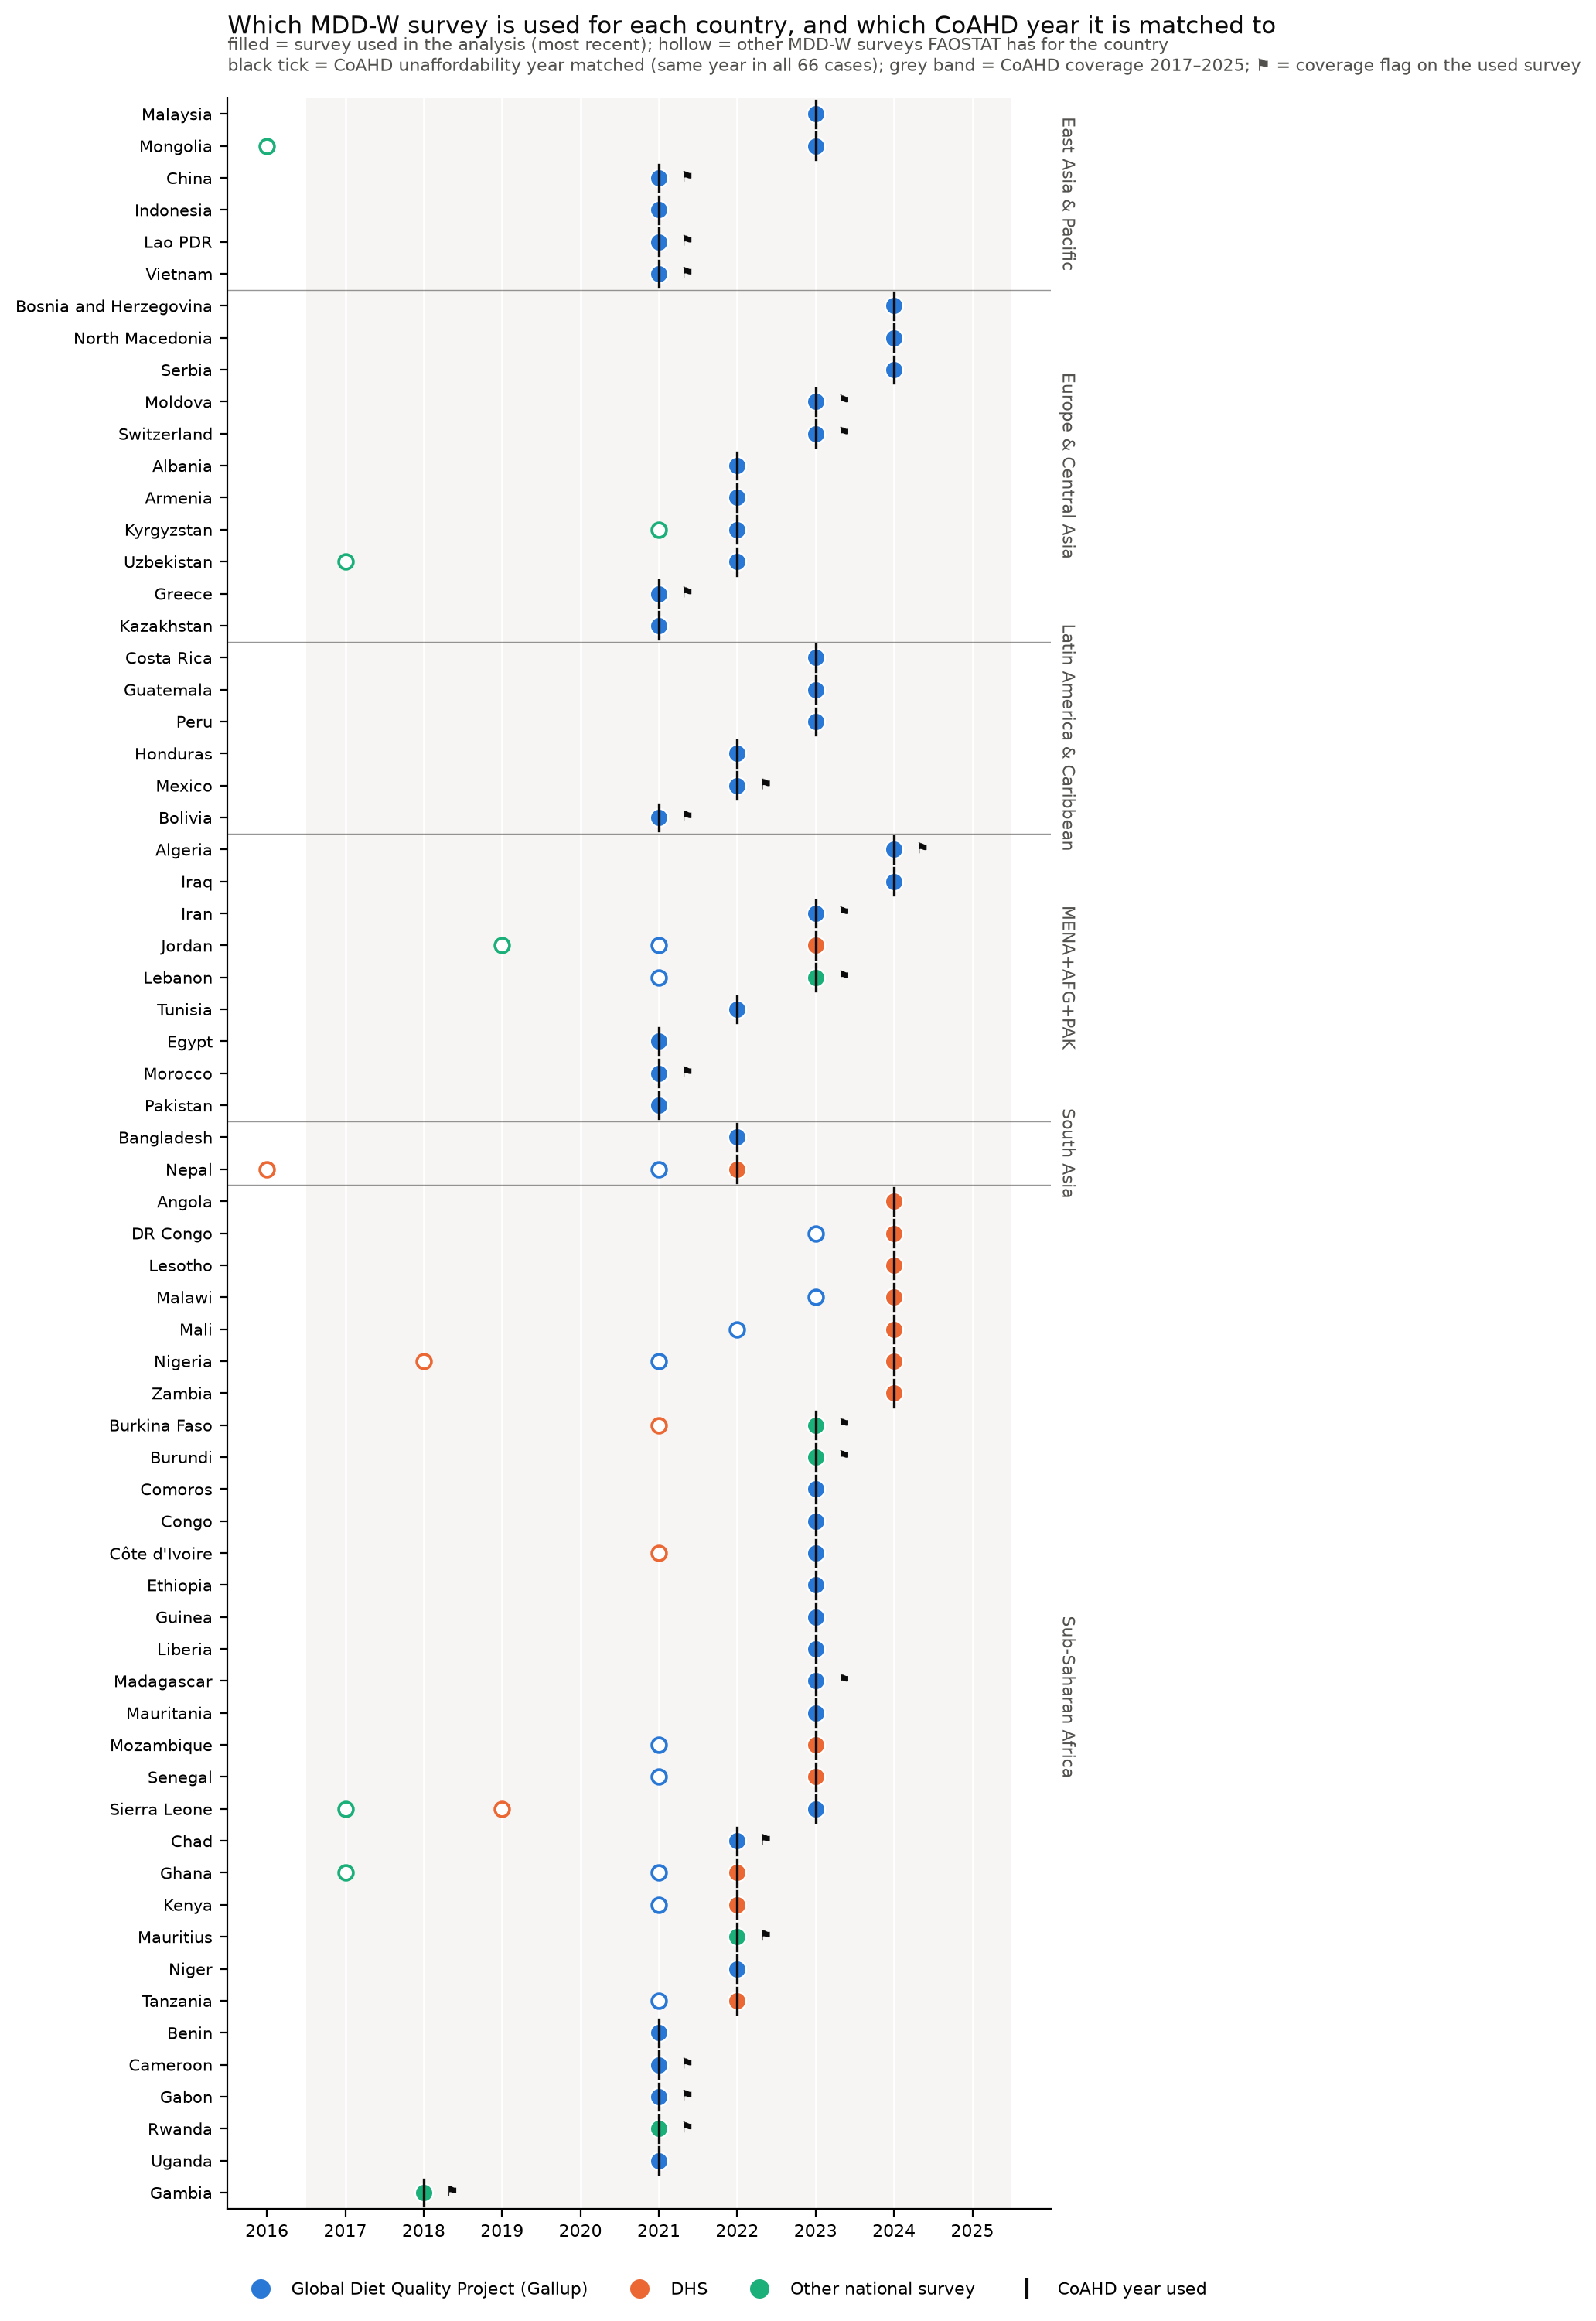
\includegraphics[width=.78\textwidth]{fig3_survey_provenance.png}
\caption{Survey provenance for the 66-country panel. Filled markers denote the survey used (most recent per country); hollow markers denote other surveys available in the SDG 2.2.4 series; the black tick marks the matched CoAHD year (identical to the survey year in all 66 cases); flags mark surveys with a documented coverage limitation.}
\label{fig:provenance}
\end{figure}

\section{Additional sensitivity tests}\label{app:sens}

Seven further sensitivity tests probe analytic choices rather than substantive objections; none alters any conclusion. The purpose of each is as follows.

\begin{itemize}
\item \emph{Fractional logit.} MDD-W is a share bounded between 0 and 100, and OLS can in principle predict outside that range; a quasi-binomial GLM with a logit link respects the bounds. Its residuals rank countries identically to OLS ($\rho=0.99$), so the linear model is retained for interpretability.
\item \emph{Restricted cubic spline (4 df).} Both variables are bounded percentages, so the relationship could bend rather than run straight. The spline does not improve on the line ($F$-test vs.\ linear, $p=0.18$).
\item \emph{Log GDP per capita alone.} A reference point for Section~\ref{sec:income}: how much would income alone explain? ($R^2=0.62$, against $0.65$ for affordability alone and $0.71$ jointly.)
\item \emph{DHS/national-sourced only.} The complement of the GDQP-only test: the relationship re-estimated on household-survey estimates alone. The subsample is small ($n=20$) but reproduces the headline slope almost exactly.
\item \emph{Precision-weighted WLS.} Gallup rounds interview roughly 300--450 eligible women where a DHS interviews more than ten thousand; weighting by the inverse of an approximate binomial variance checks that the noisiest estimates are not steering the fit. The weights rest on documented but assumed effective sample sizes, which is why this test is reported here rather than in the main text.
\item \emph{Latest-year PUA.} Replaces the survey-year CoAHD match with the most recent (2025) estimate for every country, testing whether the year-matching rule matters.
\item \emph{Drop Cook's $D>4/n$.} Removes the two most influential observations (Indonesia and Malaysia) to confirm that no single extreme country creates the slope; the leave-one-country-out test in the main text is the stricter, systematic version of this check.
\item \emph{Source-priority panel.} Rebuilds the panel preferring a DHS or national survey over Gallup wherever both exist (three countries change), testing the survey-selection rule itself.
\end{itemize}

\begin{table}[htbp]
\centering\small
\caption{Additional sensitivity tests. Columns as in Table~\ref{tab:robust}.}
\label{tab:sensx}
\begin{tabular}{lrrrrr}
\toprule
Sensitivity test & $n$ & PUA coef. & (SE) & $R^2$ & $\rho$(resid)\\
\midrule
Fractional logit (logit scale) & 66 & $-0.033$ & (0.003) & --- & 0.99\\
Restricted cubic spline (4 df) & 66 & \multicolumn{2}{c}{$F$ vs linear $p=0.18$} & 0.67 & 0.96\\
Log GDP only (log GDP coef.) & 66 & $19.2$ & (1.7) & 0.62 & ---\\
DHS/national-sourced only & 20 & $-0.69$ & (0.10) & 0.74 & ---\\
WLS, precision-weighted & 66 & $-0.69$ & (0.09) & 0.76 & 0.999\\
Latest-year PUA & 66 & $-0.71$ & (0.05) & 0.68 & 0.98\\
Drop Cook's $D>4/n$ (2 dropped) & 64 & $-0.76$ & (0.05) & 0.72 & ---\\
Source-priority panel & 66 & $-0.70$ & (0.06) & 0.65 & 0.99\\
\bottomrule
\end{tabular}
\end{table}

\section{Countries excluded from the panel}\label{app:dropped}

Thirteen countries have an MDD-W estimate but no usable CoAHD match: Afghanistan, Georgia, Libya, Timor-Leste, Ukraine, Vanuatu, and Venezuela (no CoAHD estimate at all); Cambodia, Oman, Somalia, Tajikistan, Thailand, and Zimbabwe (no CoAHD estimate within two years of the MDD-W survey).

\end{document}
